%-------------------------------------------------------------------------------
% File: simulator.tex
%       Epidemic Broadcast project documentation.
%
% Author: Marco Pinna, Rambod Rahmani, Yuri Mazzuoli
%         Created on 05/12/2020
%-------------------------------------------------------------------------------
\chapter{Simulator}\label{simulator}
In order to obtain experimental results for the presented scenarios, a simulator
was built using OMNeT++ with the support of the INET framework. This allowed us
to reproduce the different scenarios, presented in the previous chapters, with
different values for the identified parameters.\\
\section{Omnet++ and INET framework}
OMNeT++ is an extensible, modular, component-based C++ simulation library and
framework, primarily for building network simulators\footnote{https://omnetpp.org/}.\\
The INET Framework is an open-source model library for the OMNeT++ simulation
environment. It provides protocols, agents and other predefined models for
researchers and students working with communication networks. INET is especially
useful when designing and validating new protocols, or exploring new or exotic
scenarios\footnote{https://omnetpp.org/download-items/INET.html}.\\
\\
OMNeT++ is a library and a framework, and can be used with the dedicated IDE.
Not only it allows for development of the simulator itself, but also to export
simulation results and to inspect simulation behaviour with a graphical user
interface. By taking advantage of the C++ compiler optimizations, it can achieve the lowest
%riformulare o spostare ?
% inoltre 'the lowest possible' forse è un po' azzardato da scrivere
% dato che non possiamo provare che non ci siano altri modi più veloci
simulation duration possible.

Networks are composed by modules; there are two
types of modules: simple module and compound module (which can contain other
modules itself).
INET, on the other hand, is an extension of OMNeT++, dedicated to recreating 
network simulation environments, with the capability of reproducing the activity
of a wireless communication system across multiple nodes. It contains ready to
use definitions and implementations of network related modules.\\
The INET framework was chosen in order to avoid spending too
much time on the coding side and therefore be able to focus more on other
aspects such as the problem modelling and analysis.
\section{Network architecture}
The network based architecture is composed by an array of \texttt{Host} modules, an
\texttt{Integrated visualizer} (visualizer) and a \texttt{UnitDiskRadioMedium} (radioMedium);
\begin{figure}[H]
    \begin{center}
        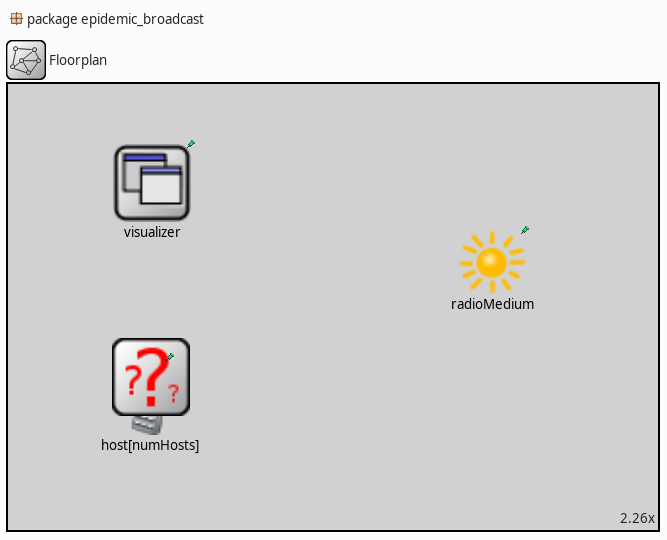
\includegraphics[scale=0.35]{img/floorplan.png}
        \caption{Floorplan.ned}
        \label{fig:floorplanOmnet}
    \end{center}
    \vspace*{-0.8cm}
\end{figure}
\begin{itemize}
    \item \textbf{UnitDiskRadioMedium} is a compound module provided by INET.
    This radio medium model provides a very simple but fast and predictable
    physical layer behaviour. It must be used in conjunction with the
    \texttt{UnitDiskRadio} model. It can simulate the behaviour of the wireless
    communication channel with various levels of abstraction.
    \item \textbf{Integrated visualizer} is a compound module provided by INET.
    It's resposible for the visual representation of modules properties and
    events in the graphic user interface.
    \item \textbf{Host} is the compound module developed to represent a node
    in the network environment.
\end{itemize}
The \texttt{Host} module extends the NodeBase module defined by INET. This
module contains the most basic infrastructure for network nodes that is not
strictly communication protocol related. The following diagram shows usage
relationships between types:
\begin{figure}[H]
    \begin{center}
        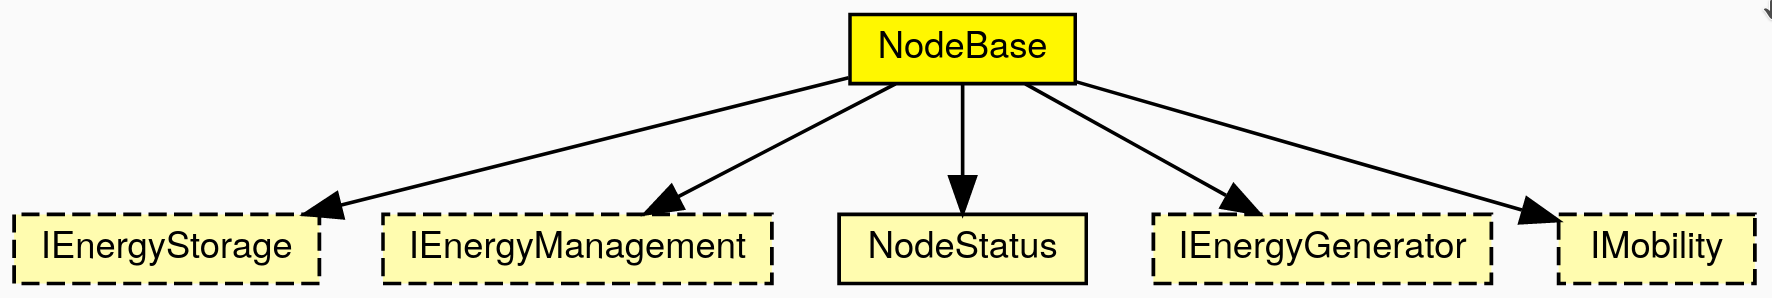
\includegraphics[scale=0.26]{img/nodebase.png}
        \caption{NodeBase Diagram.}
        \label{fig:nodebaseOmnet}
    \end{center}
    \vspace*{-0.8cm}
\end{figure}
\begin{figure}[H]
    \begin{center}
        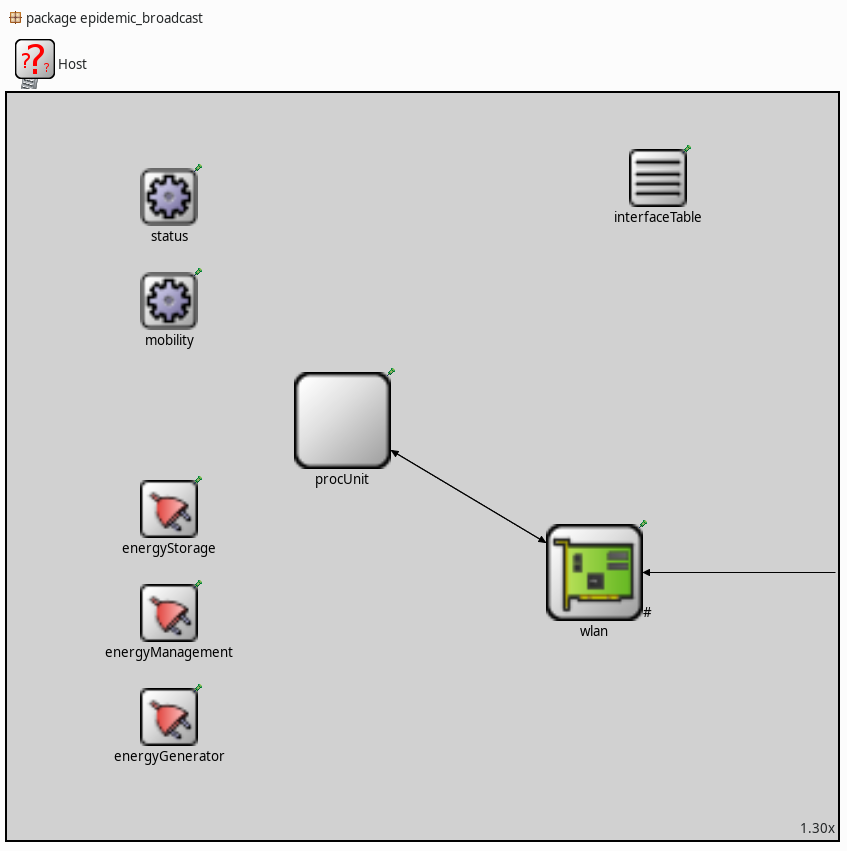
\includegraphics[scale=0.35]{img/host.png}
        \caption{host.ned}
        \label{fig:hostOmnet}
    \end{center}
    \vspace*{-0.8cm}
\end{figure}
\begin{itemize}
    \item the \texttt{mobility} module privided by INET manages the position of
    the parent module \texttt{Host}; it allows various types of movements, but
    in this study was only used for the initial random placement of the
    nodes. After being placed, all nodes are stationary for the whole duration of the simulation.
    \item the \texttt{interfaceTable} module is provided by INET and is required
    for correct operation of the radioMedium module.
    \item the \texttt{wlan} module is the wireless interface that allows nodes
    to communicate with each other. It is an \texttt{AckingWirelessInterface}
    compound module, which is the simplest wireless interface provided by INET.
    \item the \texttt{status} module is provided by INET as well and is required
    to shut down and restart network interfaces.
    \item the \texttt{procUnit} module is the custom made processing unit, that
    implements the node behaviour when a message arrives. It is connected to the
    \texttt{wlan} module in order to be able to receive and send messages.
    \item \texttt{energyStorage}, \texttt{energyManagement} and
    \texttt{energyGenerator} are modules inherited from \texttt{NodeBase} but
    they are not instantiated as there was no need to model energy-related
    behaviours.
\end{itemize}
The \texttt{wlan} module is in charge of checking each and every message for
collisions, and drop broken packets instead of forwarding them to the processing
unit. The processing unit \texttt{ProcUnit} implements the behaviours of the
nodes; it handles the broadcast message when received, and then its
retransmission when the random variable extraction results in a success. Finally
it shuts down the network interface, preventing it from receiving any messages
or provoking collisions. The network interface is turned off also for the entire
duration of the RV extractions.
\section{Parameters and statistics}
During the simulation, signals are used to collect the statistics. They are all
collected by the \texttt{Floorplan} module:
\begin{itemize}
    \item The \texttt{wlan} module emits a signal every time a collision is
    detected; this signal is collected by the
    \texttt{packetDropIncorrectlyReceived} statistic of the same module; we are
    interested in the total number of collisions detected by each node.
    \item The \texttt{ProcUnit} module emits $2$ signals when initialized,
    \texttt{hostX} and \texttt{hostY}, collected, respectively, by the
    \texttt{hostXstat} and \texttt{hostYstat} statistics; those are the
    coordinates of the parent node in the floorplan.
    \item The \texttt{ProcUnit} module emits the \texttt{timeCoverage} singal as
    well, collected in the \texttt{timeCoverageStat} statistic; this is a
    vector containing, for each node that received the broadcast message, the
    number of the time slot when the broadcast message was actually received; at
    the end of the simulation, its size represents the number of covered nodes.
\end{itemize}
Most significant parameters set up in the initialization file
(\texttt{floorplan.ini}) are reported below:
%TODO remove? p=1 is just a place-holder which gets replaced
% during initialize of every procUnit, it's not really significant
\begin{itemize}
    \item \texttt{Floorplan.host[*].procUnit.slotLength = 1}
    \item \texttt{Floorplan.host[*].procUnit.p = 1}
\end{itemize}
%snapshot del file ini con gli sweep per p ed r, e altri parametri più significativi 
\section{Design Choices and Optimizations}
Using the INET framework for the development of the simulator allowed for the use of pre-built modules for modelling wireless communications; for example,
collision detection and statistics collection are already implemented by INET
modules. During the development we choose for every aspect the optimal level of
abstraction for our purposes, but it is possible to model other aspects just 
changing the types of INET modules used, or by adding new ones. We voluntarily
avoided taking into account phenomena like path loss and node movement, and we 
restricted our considerations to a discrete time scenario. However, modelling
continuous time scenarios can be done easily by changing few INET modules types
and attributes.\\
INET modules also have pre-built optimization structures, that become
indispensable when the number of hosts becomes larger; in order to make the
simulator ready for high complex scenarios we used the \texttt{neighborCache}
structure offered by the \texttt{radioMedium} module. This module is in charge
of storing proximity information of each and every node, in order to speed up
message delivery. By setting the type of this module to \texttt{GridNeighborCache},
it is possible to reduce the time needed for a simulation with more than
$2000$ devices dropped on the floorplan, by a factor of $10$; we also found that
this type of cache (with the right value for the \texttt{cellSize} parameter) is
the best trade-off between speed and memory occupancy, for this type of
workload\footnote{https://doc.omnetpp.org/inet/api-current/neddoc/inet.physicallayer.contract.packetlevel.INeighbor\\
Cache.html}.  

\section{Validation}
To ensure the correctness of the simulator and the meaningfulness of the results, the simulator has been validated by means of two simplified scenarios, namely the single queue configuration and the star configuration, which are discussed in \ref{ssec:singlequeue} and \ref{ssec:star2} respectively.

\subsection{Single queue validation}

\begin{figure}[H]
    \begin{center}
        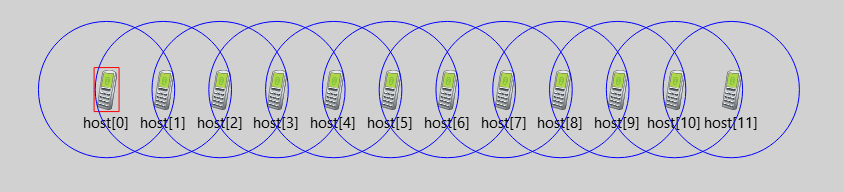
\includegraphics[scale=0.75]{img/singleQueueGUI.png}
        \caption{Validation configuration with 12 hosts placed on a line}
        \label{fig:single_queueGUI}
    \end{center}
    \vspace*{-0.8cm}
\end{figure}

In this configuration, host[0] always broadcasts during the first slot and then the message travels along the queue, with a total of 10 hops. On every hop, the per-slot probability of successful transmission is $p$, which implies an average number of attempts equal to $\frac{1}{p}$. Therefore, the expected coverage time is

\begin{equation}
    E[T] = 1 + 10 \cdot \frac{1}{p}
    \label{eq:singleQueueValidationAvgT}
\end{equation}

Validation was performed with 9 different configurations, one for  each value of $p$ ranging from $0.1$ to $0.9$, with 200 repetitions each.
The following results were obtained:
%TODO replace with plot? Better than table?

\begin{center}
\begin{tabular}{ | m{1cm} | m{5cm}| m{5cm} | }
\hline
$p$& Expected value & Experimental value (mean, interval for 95\% confidence)\\
\hline
$0.1$&$101.0$&$\textbf{99.68}, 95.55, 103.81$\\
\hline
$0.2$&$51.0$&$\textbf{49.9}, 47.93, 51.86$\\
\hline
$0.3$&$34.33$&$\textbf{34.17}, 32.88, 35.46$\\
\hline
$0.4$&$26.0$&$\textbf{25.79}, 24.93, 26.65$\\
\hline
$0.5$&$21.0$&$\textbf{20.84}, 20.24, 21.44$\\
\hline
$0.6$&$17.67$&$\textbf{17.42}, 17.0, 17.84$\\
\hline
$0.7$&$15.29$&$\textbf{15.2}, 14.87, 15.52$\\
\hline
$0.8$&$13.5$&$\textbf{13.48}, 13.25, 13.72$\\
\hline
$0.9$&$12.11$&$\textbf{12.14}, 11.97, 12.3$\\
\hline
\end{tabular}
\end{center}

As can be seen in the table above, %add label to table and reference it?
the experimental results are consistent with the theoretical expected value, with a 95\% confidence level. %rephrase?
\subsection{Star 5-to-1 validation}


\begin{wrapfigure}{r}{0.45\textwidth}
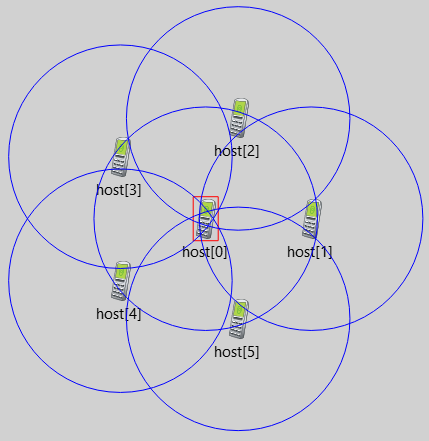
\includegraphics[width=1\linewidth]{img/omnetStar5to1.png} 
\caption{Validation configuration with 5 hosts placed on a star and a target in the middle}
\label{fig:star5to1GUI}
\end{wrapfigure}

In this configuration, host[0] is the target to be reached by the broadcast while all the others already have the message and try to broadcast at every slot with probability $p$.

This system can be modelled by a discrete-time Markov chain, as explained in \ref{ssec:star2}.
The probability of the system to be in the $i$-th state during the $j$-th slot is given by taking the $j$-th power of the stochastic matrix and taking the $i$-th element of the first row.

Validation was performed with 4 different configurations, one for each value of $p$ ranging from $0.2$ to $0.8$ with steps of $0.2$, with 1000 repetitions each.\\
For each configuration, data about the state of the system was recorded and statistics were computed, yielding experimental probabilities. These probabilities were then compared with theoretical predictions, obtained by taking powers of the appropriate stochastic matrix.\\
All the experimental results proved to be consistent with theoretical computations.

\begin{figure}[H]
    \begin{center}
        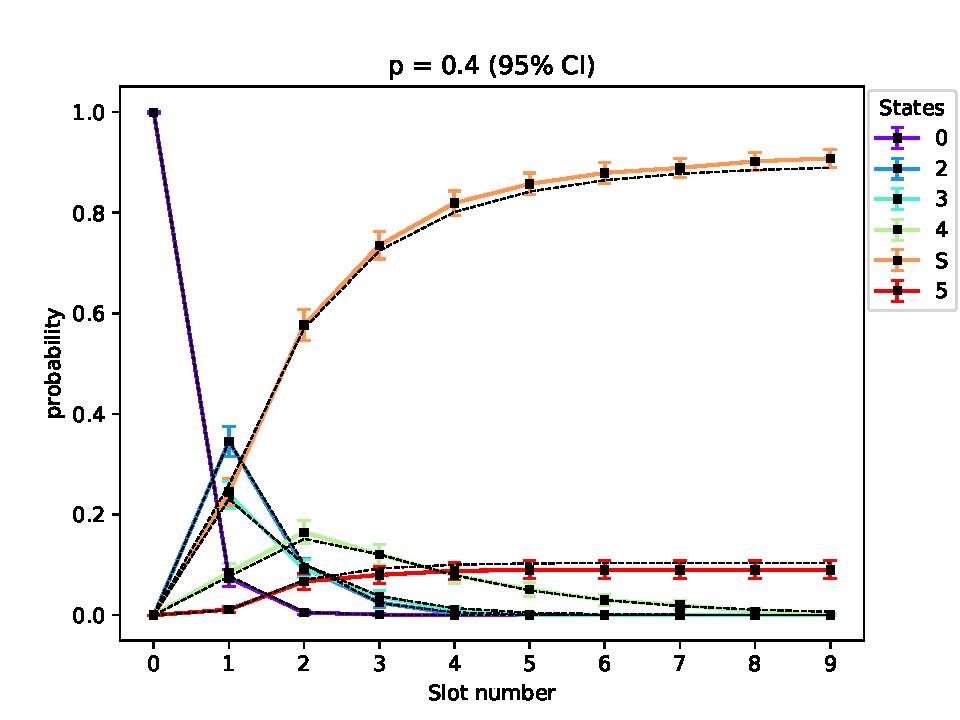
\includegraphics[scale=0.73]{img/star5to1p=0.4validation.pdf}
        \caption{Validation data for p = 0.4}
        \label{fig:5to1validPlot1}
    \end{center}
    \vspace*{-0.8cm}
\end{figure}

%TODO boh c'è spazio, ne ho messo due ma volendo se ne può lasciare solo una
%TODO there's room for two images, we can keep just one if we want

\begin{figure}[H]
    \begin{center}
        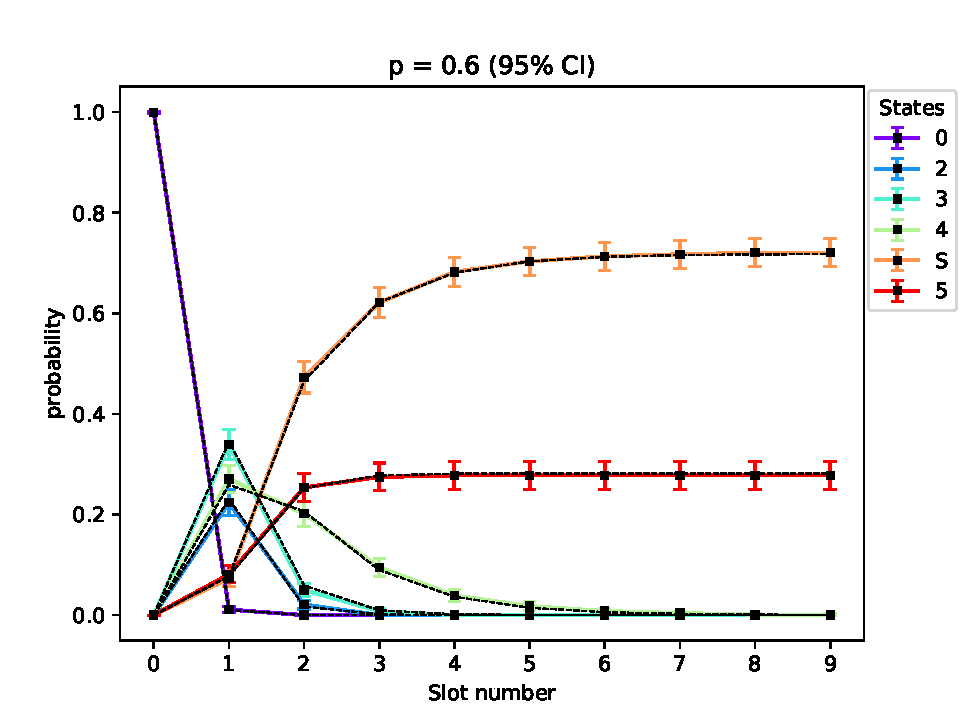
\includegraphics[scale=0.73]{img/star5to1p=0.6validation.pdf}
        \caption{Validation data for p = 0.6}
        \label{fig:5to1validPlot2}
    \end{center}
    \vspace*{-0.8cm}
\end{figure}

Figures \ref{fig:5to1validPlot1} and \ref{fig:5to1validPlot2} show graphs of the experimental data (coloured solid lines) along with predictions (black dashed lines).
%TODO remove empty blank page betwee chapter 4 and 5